\documentclass[11pt,letterpaper]{article}
\usepackage[lmargin=1in,rmargin=1in,tmargin=0.75in,bmargin=1in]{geometry}

% -------------------
% Packages
% -------------------
\usepackage{
	amsmath,			% Math Environments
	amssymb,			% Extended Symbols
	enumerate,		% Enumerate Environments
	graphicx,			% Include Images    
	lastpage,			% Reference Lastpage
	multicol,			% Use Multi-columns
	multirow,			% Use Multi-rows
	siunitx
}

\graphicspath{{./images/}}

\usepackage{wrapfig}

% -------------------
% Font
% -------------------
\usepackage[T1]{fontenc}
\usepackage{charter}    


% -------------------
% Heading Commands
% -------------------
\thispagestyle{empty}
\vspace*{-0.5in}

% -------------------
% Commands
% -------------------

\newcommand{\pspace}{\par\vspace{\baselineskip}}
\newcommand{\ds}{\displaystyle}

% -------------------
% Content
% -------------------

\begin{document}
\begin{minipage}{\textwidth}
     \begin{center}
          \textbf{\huge MATHCOUNTS Cheat Sheet}
          \vspace{0.1in}
     \end{center}
\end{minipage} \\
\rule[2ex]{\textwidth}{2pt} 
\centering
\begin{minipage}{\textwidth}
     \section*{Test Taking Strategies}
     \begin{itemize}
          \item Be sure to always make an attempt
          \item Don't be afraid to skip a question and return later
          \item Substitute in answer choices
          \item Use smaller cases to find a pattern
          \item Use tools
          \begin{itemize}
               \item Rulers, compasses, and protractors can be used to draw and estimate lengths/angle measures. Diagrams in problems are not drawn to scale.
               \item Use graph paper to model equations to determine possible solutions
          \end{itemize}
          \item Eliminate incorrect answers
          \begin{itemize}
               \item Narrow down possible answers
               \item Increases probability of guesswork
          \end{itemize}
          \item Guess! 
          \begin{itemize}
               \item Never leave a question blank
               \item There is no penalty for incorrect answers
          \end{itemize}
     \end{itemize}
     \vspace{0.5cm}
\end{minipage}
\begin{minipage}{\textwidth}
     \section*{Guessing Strategies}
     \begin{itemize}
          \item Sometimes you can eliminate
          \begin{itemize}
               \item Answer choices too large or small
               \item Answer choices odd or even
               \item Answer choices divisible by $x$
          \end{itemize}
          \item In geometry problems, estimate the dimensions
          \begin{itemize}
               \item Graph paper, rulers, and protractors are allowed; draw your own diagrams!
               \item Divide the shape into subsections and estimate the values of each portion
          \end{itemize}
        \end{itemize}
        \vspace{0.5cm}
\end{minipage}
\begin{minipage}{\textwidth}
     \section*{Common Situations/Vocabulary}
     \begin{itemize}
          \item Mean: the average value for a data set = $\frac{\text{Sum of all Terms}}{\text{Number of Terms}}$
          \item Median: the point in the middle of a data set; exactly 1/2 on either side
          \item Mode: the most common number in a data set
          \item Speed: $\frac{Distance}{Time}$
          \item Distance: $Speed \times Time$
          \item Combinations: formula to choose $k$ objects from $n$ =${{n}\choose{k}} = \frac{n!}{k!(n-k)!}$
     \end{itemize}
\end{minipage}

\newpage

\begin{minipage}{\textwidth}
     \section*{Geometry}
     \begin{center}
          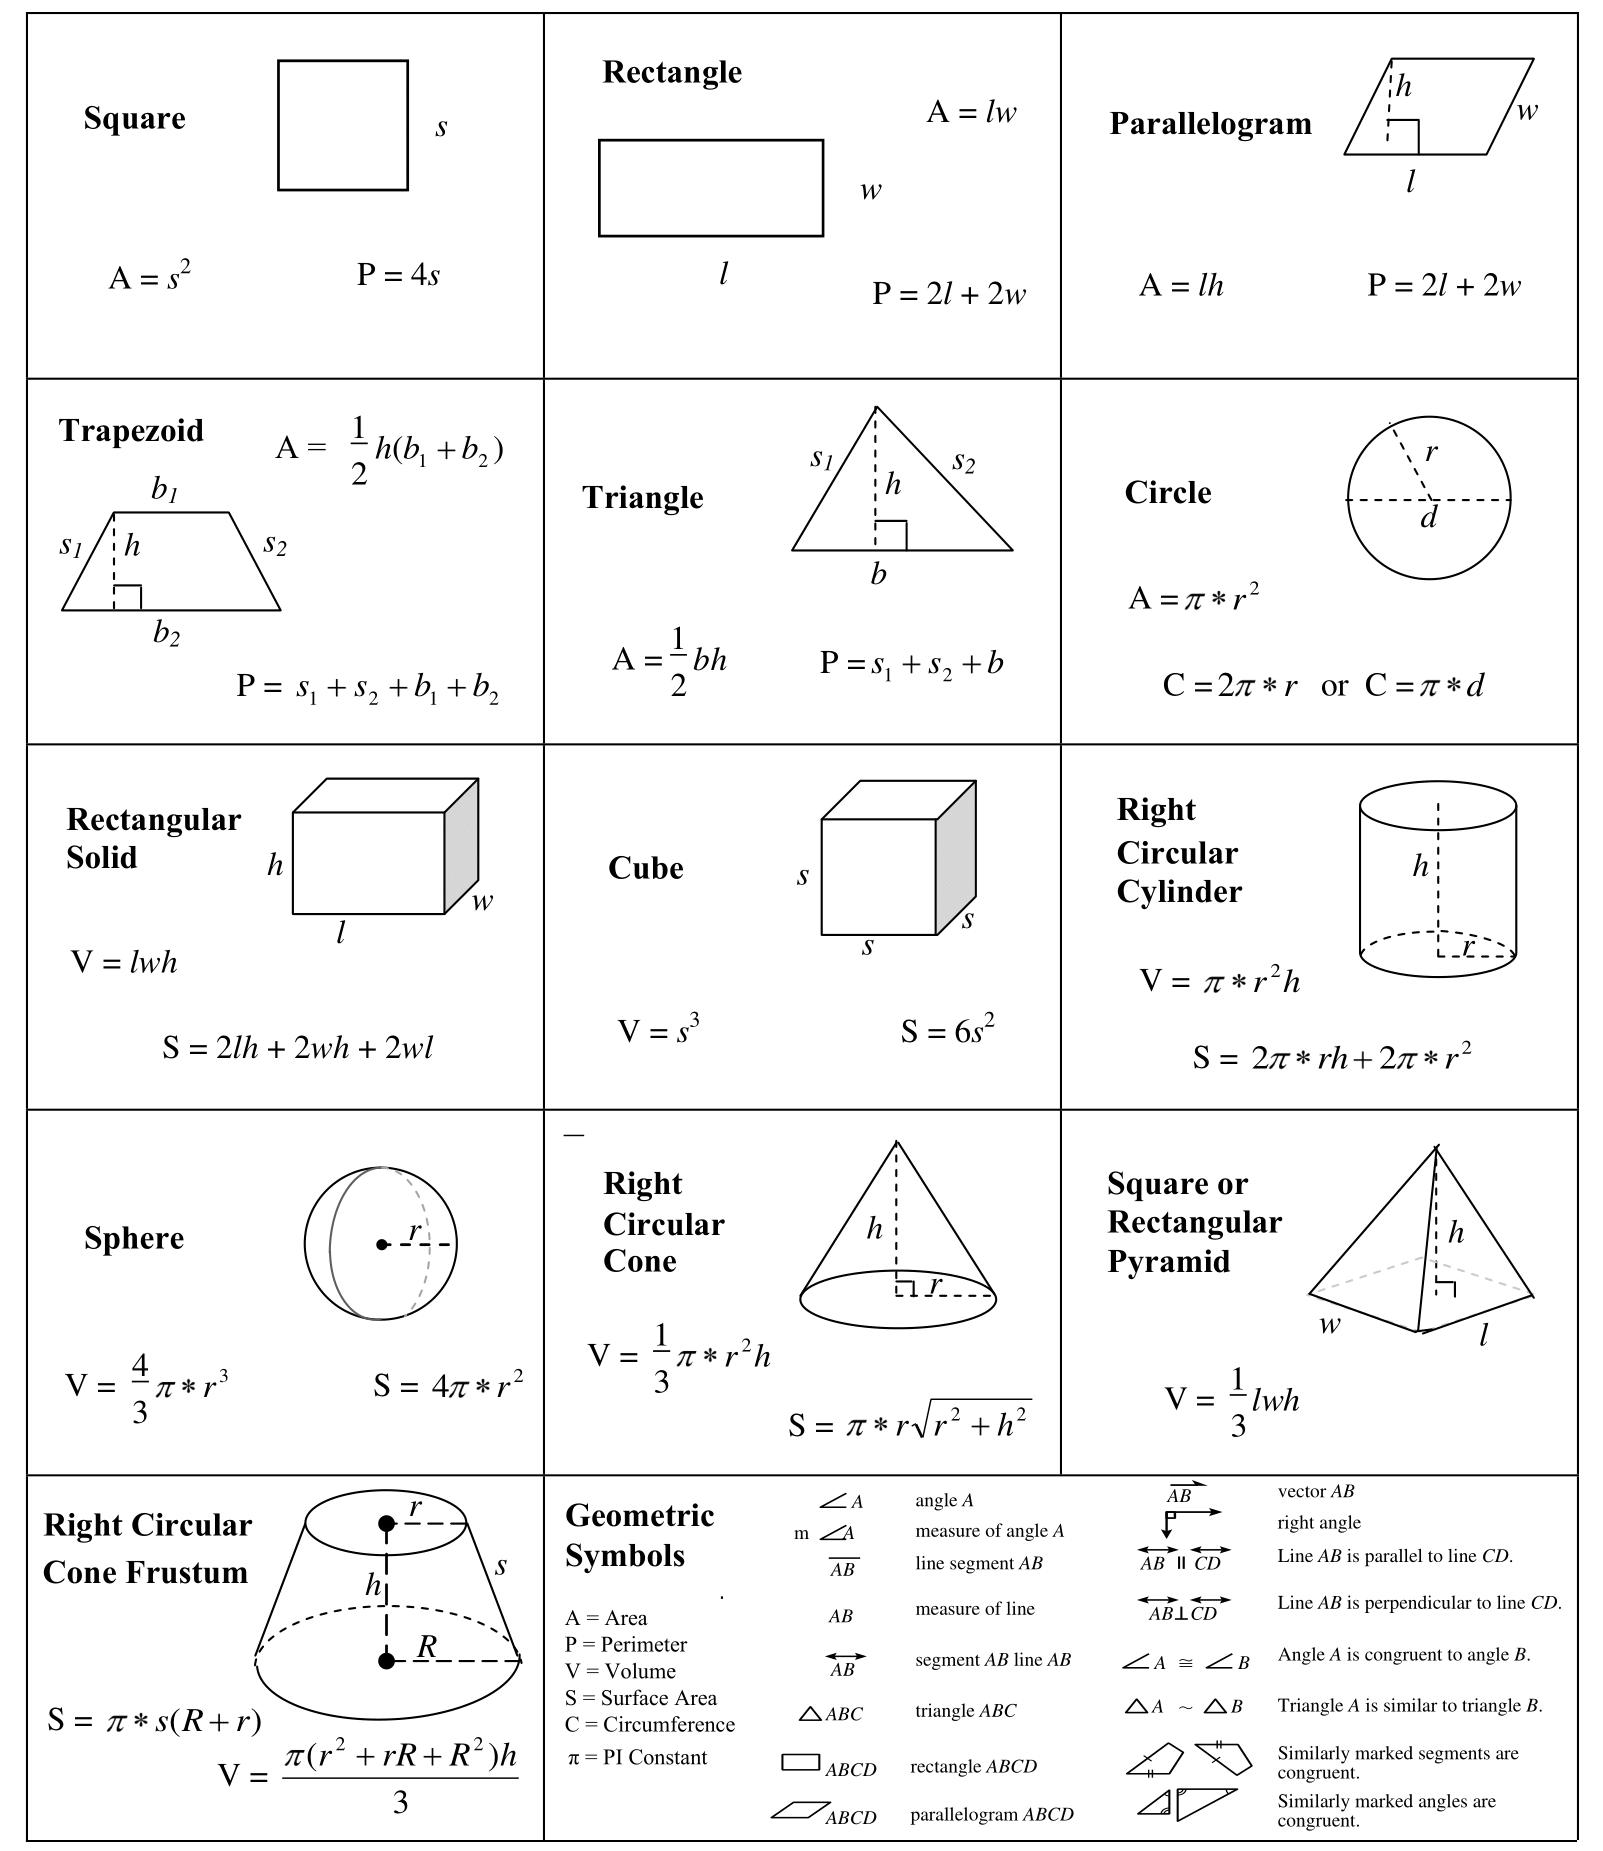
\includegraphics[height = 20cm]{images/geometry.png}
     \end{center}    
\end{minipage}
\begin{minipage}{\textwidth}
     \begin{itemize}
          \item Angle Pair Relationships
          \begin{itemize}
               \item Adjacent Angles: angles that neighbor each other bisected by a single line
               \item Complementary Angles: angles that add up to $90^{\circ}$
               \item Supplementary/Linear Angle Pairs: angles that add up to $180^{\circ}$ along a straight line
               \item Vertical Angles: pairs of opposite angles made by two intersecting lines
               
               \vspace{0.2cm}
               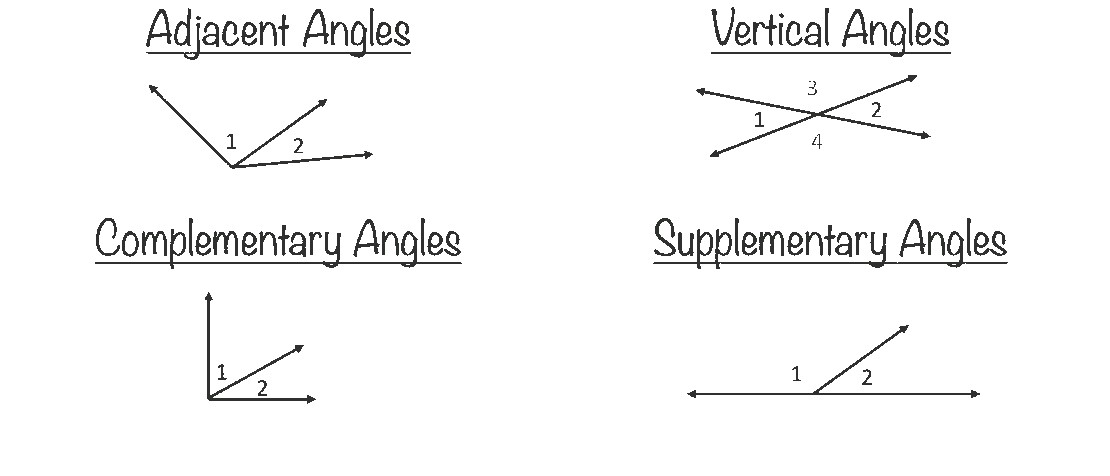
\includegraphics[height = 7cm]{images/anglrel.jpg}
          \end{itemize}
          \vspace{-0.5cm}
          \item Triangles
          \begin{itemize}
               \item When a triangle has an angle of $90^{\circ}$, the sum of the squared legs is equal to the squared hypotenuse; $a^2+b^2=c^2$
               \item The numbers that are possible for the values of $a$, $b$, and $c$ are known as Pythagorean triples. Common triples include:
               \begin{itemize}
                    \item $3$, $4$, $5$
                    \item $5$, $12$, $13$
                    \item $6$, $8$, $10$
                    \item $7$, $24$, $25$
                    \item $9$, $12$, $15$
               \end{itemize}
          \end{itemize}
          \item Circles
          \begin{itemize}
               \item Area of a Sector = $\dfrac{\pi r^2\theta}{360^{\circ}}$
               \item Length of an Arc = $\dfrac{2\pi r\theta}{360^{\circ}}$
          \end{itemize}
          \item Polygons
          \begin{itemize}
               \item Sum of the Interior Angles of a Polygon = $(\text{number of sides}-2) \times 180$
               \item Measure of an Interior Angle of a Regular Polygon = $\dfrac{n-2}{n} \times 180$
               \item Measure of an Exterior Angle of a Regular Polygon = $\dfrac{360}{n}$
          \end{itemize}
        \end{itemize} 
\end{minipage}

\begin{minipage}{\textwidth}
     \section*{Systems of Equations}
     A system of equations is a set of equations which share the same variables.
     \begin{itemize}
          \item Elimination
          \begin{itemize}
               \item  Elimination involves removing variables from the system by adding constant multiples of two or more of the equations together.
               \subsection*{Example}
               Find the ordered pair $(x,y)$ for which
               \[\left\{\begin{array}{l}x-12y=2\\3x+6y=6\end{array}\right.\]
               \subsection*{Solution}
               We can eliminate $y$ by adding two times the second equation to the first:
               \[x - 12y + 2(3x+6y)= 2 + 2(6).\]
               Simplifying
               \[7x + 0=14.\]
               So, $x=2$. Then, we can plug in for $x$ in either of the equations:
                    \begin{align*} 
                         2-12y &= 2 \\ 
                         y &= 0 
                    \end{align*}
          \end{itemize}
          \item Substitution
          \begin{itemize}
               \item Substitution requires solving for a variable and then plugging that variable into another equation, therefore reducing the number of variables.
               \subsection*{Example}
               Find the ordered pair $(x,y)$ for which
               \[\left\{\begin{array}{l}x-12y=2\\3x+6y=6\end{array}\right.\]
               \subsection*{Solution}
               Solving the first equation for $x$:
               \[x = 12y + 2.\]
               Plugging this into the second equation:
               \[3(12y + 2) + 6y = 6 \Leftrightarrow 42 y = 0.\]
               Thus, $y=0$. Plugging this into either equation and solving for $x$ yields $x=2$.
          \end{itemize}
     \end{itemize}
\end{minipage}
\begin{minipage}{\textwidth}
     \section*{Special Factorizations}
     $a^2 +2ab+b^2 = (a+b)^2$ \\ 
     $a^2 - 2ab+b^2 = (a-b)^2$ \\
     $a^3 +3a^2b+3ab^2 +b^3 = (a+b)^3$ \\
     $a^3 -3a^2b+3ab^2 -b^3 = (a-b)^3$ \\
     $a^2 -b^2 =(a+b)(a-b)$ \\
     $a^3 +b^3 =(a+b)(a^2 -ab+b^2)$ \\
     $a^3 -b^3 =(a-b)(a^2 +ab+b^2)$
     \vspace{0.5cm}
\end{minipage}
\begin{minipage}{\textwidth}
     \section*{Divisibility Rules}
     2 → iff units digit is even \\ 
     3 → iff sum of digits is divisible by 3 \\
     4 → iff last two digits form a number divisible by 4 \\
     5 → iff units digit is 0 or 5 \\
     6 → iff number is divisible by both 2 and 3 \\
     7 → iff result of subtracting twice the last digit from the number remaining when the last digit is removed is divisible by 7 \\
     8 → iff last three digits of number form a number divisible by 8 \\
     9 → iff sum of digits is divisible by 9 \\
     10 → iff units digit is 0 \\
     11 → iff result of alternately adding and subtracting the digits is divisible by 11 \\
     12 → iff number is divisible by both 4 and 3 \\
     
     You can combine the divisbility rules of factors to determine the divisibility of any multiple! Note that the rules for 6 and 12 utilize this principle.
     \vspace{0.5cm}
\end{minipage}
\begin{minipage}{\textwidth}
     \section*{Units Digits Patterns} 
     When we have a sequence $\{a_0, a_1, a_2, \ldots\}$ where the unit digit of $a_0$ is any of the following digits, then the unit digits of $a_1, a_2, a_3, \ldots$ will follow this pattern. \\ 
     \vspace{0.05cm}
     
     $1 \rightarrow 1$ \\
     $2 \rightarrow 2,4,8,6$ \\
     $3 \rightarrow 3,9,7,1$ \\
     $4 \rightarrow 4, 6$ \\
     $5 \rightarrow 5$ \\
     $6 \rightarrow 6$ \\
     $7 \rightarrow 7,9,3,1$ \\
     $8 \rightarrow 8,4,2,6$ \\
     $9 \rightarrow 9, 1$ \\
\end{minipage}
\begin{minipage}{\textwidth}
     \section*{Arithmetic Series}
     \begin{itemize}
          \item An arithmetic sequence is a sequence of numbers such that the \underline{difference} between any two consecutive terms is constant.
          \begin{itemize}
               \item For example, $1, 2, 3, 4$ is an arithmetic sequence with a common difference $1$, and $115, 110, 105, 100$ is an arithmetic sequence with a common difference $-5$
               \item $1, 2, 3, 5, 10$ is not an arithmetic sequence because the difference between consecutive terms varies
          \end{itemize}
          \item The \underline{arithmetic series} is the sum of all the terms in an arithmetic sequence
          \begin{itemize}
               \item The formula is $\dfrac{n}{2}(a_1+a_n)$ where $n$ is the number of terms, $a_1$ is the first term, and $a_n$ is the last term
          \end{itemize} 
     \end{itemize}
     \section*{Geometric Series}
     \begin{itemize}
          \item A geometric sequence is a sequence of numbers such that the \underline{ratio} between any two consecutive terms is constant. This constant is called the common ratio of the sequence.
          \begin{itemize}
               \item For example, $1, 2, 4, 8$ is a geometric sequence with a common ratio $2$ and $100, -50, 25, -25/2$ is a geometric sequence with a common ratio $-1/2$
               \item $1, 3, 9, -27$ and $-3, 1, 5, 9, \ldots$ are not geometric sequences, as the ratio between consecutive terms varies
               \item More formally, the sequence $a_1, a_2, \ldots , a_n$ is a geometric progression if and only if $a_2 / a_1 = a_3 / a_2 = \cdots = a_n / a_{n-1}$. We can also express it as $a, ar, ar^2, \ldots$
               \item A similar definition holds for infinite geometric sequences. It appears most frequently in its three-term form: namely, that constants $a$, $b$, and $c$ are in geometric progression if and only if $b / a = c / b$.
          \end{itemize}
          \item The \underline{finite geometric series} is the sum of all the terms in a finite geometric sequence
          \begin{itemize}
               \item The formula is $\dfrac{a(r^n-1)}{r-1}$, where is $a$ is the first term, $r$ is the ratio, and $n$ is the number of terms 
          \end{itemize}
          \item The \underline{infinite geometric series} is the sum of all the terms in an infinite geometric sequence
          \begin{itemize}
               \item An infinite geometric series converges if and only if $|r|<1$
               \item If this condition is satisfied, the series converges to $\dfrac{a}{1-r}$
          \end{itemize}
     \end{itemize}
     \vspace{3em}
\end{minipage}
\end{document}
